\chapter{Software OpenSource y Libre}
%Conclusión!!Trabajar con un sistema final bajo licencias de hardware siguiendo el modelo de la Licencia LGPL para el software. Estamos comprometidos con el ideal de libre disposición, de libre uso y hardware de código abierto reutilizable.
	

\section{Software OpenSource y Libre}


		\subsection{}{Deferencias}%http://www.slideshare.net/wilberth1594/tesis-alex-8795926,julius

		\subsection{GPL}
		\subsection{LGPL}
%Revisemos este título -- PABLO JULIUS :P
		\subsection{OpenSource}

		\subsection{¿Quien tiene el Hardware?}

		\subsection{OpenRISC}
	%\subsection{Introducción}



Una interpretación sencilla de lo que se entiende por el término open source , cuando se utiliza en la
contexto de la descripción de un programa de software o diseño de hardware , es que el diseño
Fuentes de alguna manera están disponibles a la vista. A pesar de que es una amplia y potencialmente
término ambiguo , un común acuerdo sobre la definición está en un documento llamado
la Open Source Definition (OSD ), publicado por la Open Source Initiative (OSI ) .
La definición no es una licencia de software libre en sí , más bien algo para medir condiciones de distribución frente para determinar si cumplen y , si lo hacen, entonces se puede decir
a ser de código abierto ( 36 ) . Lo que no es inmediatamente claro es lo que podría o debería ser
hecho con una copia de la fuente de diseño , práctica y legalmente. Cuando el software libre
se utiliza para describir el software de código abierto , se refiere no al costo para el usuario ,
pero los derechos del usuario. La Fundación para el Software Libre (FSF ) ofrece una definición
para mostrar claramente qué debe cumplir sobre una pieza de software para que pueda ser considerado
libre ( 35 ) .
El software libre de código abierto plazo ( FOSS) se usa para referirse al software
adherirse tanto al OSD y FSD . El software libre y de código abierto es una sociedad inclusiva
término que abarca tanto el software libre y software de código abierto que , a pesar de
describir los modelos de desarrollo similares , tienen diferentes culturas y filosofías.
El software libre se enfoca en las libertades filosóficas que da a los usuarios, mientras que abierto
origen se centra en las fortalezas percibidas de su modelo de desarrollo peer-to -peer ( 37 ) ( 38 ) .


%\cite{Etiqueta02},
%\textit{FPGAs}) .


%\begin {itemize}
%\item  Bloques lógicos configurables y \textit{Lookup Tables}.
% \end {itemize}

\begin{figure}[h!]
 \begin{center}
  % 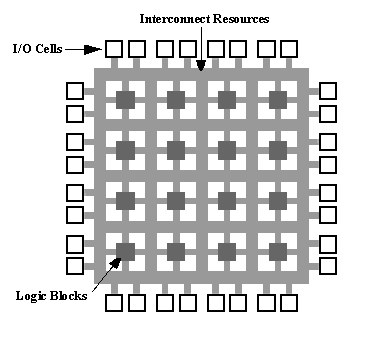
\includegraphics[width=0.5\textwidth,keepaspectratio=true]{./images/fpga1a}
  \caption{Componentes de una FPGA}
  \label{fig:esquema}
 \end{center}
\end{figure}

